% SPDX-FileCopyrightText: (c) 2026 Kush Shah
% SPDX-License-Identifier: Apache-2.0
%
% Proof -- IEEE BIBM 2026 Undergraduate & High School Symposium
% REVISED PROSE VERSION. Built from the finished PDF text, with the
% sentence-level revisions applied, US spelling throughout, noun-phrase
% section headings, and the complete 15-entry bibliography.
%
% COMPILE: Overleaf -> New Project -> Template -> "IEEE Conference".
%          Replace the .tex, upload figures/out/*.pdf, compile twice.
%
% >>> CHECK THE PAGE COUNT FIRST. The limit is 5 pages including references.
% >>> If it comes out at 6, delete in THIS ORDER until it fits:
% >>>   1. the paragraph marked [CUT FIRST]  (Section V-D, subgroup caveat)
% >>>   2. the paragraph marked [CUT SECOND] (Section I, final paragraph)
% >>> Both are additions. Everything else matches the 5-page PDF.

\documentclass[conference]{IEEEtran}
\IEEEoverridecommandlockouts
\usepackage{cite}
\usepackage{amsmath,amssymb}
\usepackage{graphicx}
\usepackage{booktabs}
\usepackage{url}
\usepackage[hidelinks]{hyperref}
\graphicspath{{figures/out/}}

\begin{document}

\title{Checking a Monotonicity Precondition in Hardware:\\
A Glycemic-Response Inference Chip for Streamed Per-Patient Weights}

\author{\IEEEauthorblockN{Kush Shah}
\IEEEauthorblockA{\textit{Del Norte High School (high school student)}\\
San Diego, USA\\
kushshah.edu@gmail.com}}

\maketitle

\begin{abstract}
A clinician can audit a model whose predicted glycemic response is guaranteed
never to fall as carbohydrate rises. Every method we know of establishes that
guarantee during training and verifies it \emph{offline, on a fixed model},
which is sound for exactly as long as the model stays fixed. We describe
\emph{Proof}, a $1\times1$-tile fixed-point inference ASIC for the IHP SG13G2
open PDK that holds no weights at all. Every weight arrives from an untrusted
host, so the model can be specific to one patient, and the offline assumption
no longer holds. The sign condition our guarantee rests on is never satisfied
by an unconstrained fit. It fails for the population model, and it fails for
all 44 held-out per-participant refits of the CGMacros cohort, across a
twentyfold range of fine-tuning budgets. Personalization does not open that
gap; what it does is make the gap undecidable offline. The chip therefore
checks its own precondition at the pin interface, for 20 flip-flops, by
carrying one sign bit and one non-zero bit per hidden unit in registers that
rotate in lockstep with the hidden activations. We also report a defect that
motivated the approach. The datapath was provably monotone internally while the
fixed-width output field truncated, so the \emph{reported} response fell from
31{,}293 to $-31{,}209$ for a one-count rise in carbohydrate at the same time
as the true value rose. The design closes at 83.53\,\% utilization with zero
DRC, LVS and antenna violations. All accuracy figures come from 45 participants
with no held-out validation set, and should be read as optimistically biased
upper bounds.
\end{abstract}

\begin{IEEEkeywords}
monotonic neural networks, hardware safety, quantized inference, glycemic
response, open-source silicon
\end{IEEEkeywords}

\section{Introduction}

People managing type~2 diabetes are routinely asked to make a comparative
judgment about food. \emph{Will this meal raise my blood sugar more than that
one?} Continuous glucose monitoring makes the answer measurable after the fact,
and a small model over meal macronutrients can estimate it beforehand. Such a
model also has to behave sensibly, which here means that adding carbohydrate
must never lower the predicted response. A model that violates this is
incoherent as advice, and no aggregate accuracy figure repairs that.

Monotonic-by-construction networks are a mature field, and certifying the
monotonicity of a trained network is well studied. Both lines of work share an
assumption worth naming. The guarantee is established during training and
checked \emph{offline}, once, against a fixed set of weights. A device that
ships with one model inherits that certificate.

Our device does not ship with one model. \emph{Proof} holds no weights at all.
Its 65 learned parameters arrive over the pins for every inference, as 74 INT8
weight and bias bytes (each bias is carried as two bytes) alongside 9
requantization shift bytes. This began as an area decision, since the
parameters do not fit beside the datapath in a $1\times1$ Tiny
Tapeout~\cite{tinytapeout} tile on the IHP SG13G2 open PDK~\cite{ihp}. The
consequence is that the weights can be \emph{specific to one patient}, and an
offline certificate covers the weight set it was computed for and no other. We
call the host untrusted in a modest sense. We do not assume it used the
constrained objective we train with, and nothing in the weight stream reveals
whether it did.

This paper makes four claims. Per-patient weights are worth having: refitting
one parameter from about eight logged meals, roughly three days of logging,
improves per-participant error by a margin whose 95\,\% interval excludes zero,
while a single meal is measurably \emph{worse} than none
(Fig.~\ref{fig:personalisation}). The precondition really does fail, and not
marginally. No unconstrained fit we tried satisfies the sign condition, neither
the population model nor any one of 44 per-participant refits. It is
nevertheless checkable in hardware for 20 flip-flops, because both operands
already cross the pins (Fig.~\ref{fig:arch}). Finally, a property of this kind
can hold internally and still break at the interface. Our datapath was provably
monotone while the output field truncated, and truncation wraps
(Fig.~\ref{fig:r4}).

None of the four is an accuracy claim. The model in Section~\ref{sec:results}
is small, the cohort is 45 people, and we do not claim it beats an
unconstrained baseline. The contribution is where the guarantee is checked, not
how well the model predicts.

\section{Related Work}

\textit{Personalized glycemic response.} Postprandial response to an identical
meal varies widely between people, and is predictable from personal
features~\cite{zeevi2015},~\cite{berry2020}. We take that premise as given and
treat its hardware consequence as our contribution.

\textit{Monotonicity, established and certified.} Architectures that guarantee
monotonicity by reparameterizing weights through a non-negative
map~\cite{runje2023},~\cite{scalable2024} form an established family. The
softplus reparameterization we train with sits squarely inside it and is not a
contribution here. Liu et al.~\cite{liu2020} take the other route, certifying a
trained network by mixed-integer programming, which is costly and runs offline
against a fixed model. They also name the predicate we check, sign
verification, and report that their certified networks often fail it. The
condition is sufficient but not necessary, so our guard is sound but not
complete: it will decline monotone weight sets that it cannot check at a pin
interface. We find no such case here. For all 44 refits the guard rejects, a
falling response exists.

\textit{Quantization versus structural guarantees.} Recent work asks whether
quantization preserves monotone-operator properties~\cite{quantmon2026}. This
is the nearest hit to ours and still distinct. It concerns monotone-operator
theory instead of input--output monotonicity, its certificate is an offline
norm bound, and it has no hardware. Formal verification of quantized
networks~\cite{qvip2022} is likewise offline, and what it verifies is the
network itself, not the interface the network arrives through.

\textit{Hardware that inspects weights.} Accelerators are commonly protected by
algorithmic checksums descended from ABFT~\cite{huang1984},~\cite{ozen2020} and
by permanent-fault schemes~\cite{zhang2018}. SoftSNN is the closest to us in
mechanism, bounding incoming weight \emph{magnitudes} against a threshold in
hardware~\cite{putra2022}. The distinction is not one of degree. Those
techniques ask whether a value was \emph{corrupted}. We ask whether an intact
weight set \emph{admits the guarantee at all}. In our failing case nothing is
corrupted: the arithmetic is perfectly correct, and every output is bit-exact
against the integer reference model. What fails is a relation \emph{between}
two weights that arrive in different layers, and no per-weight bound or
checksum can express such a relation. Run-time safety
monitoring~\cite{xiang2022} is closer in spirit, though it operates at system
level, in software, on \emph{outputs}.

To our knowledge, no prior hardware checks a semantic precondition on a
streamed weight set at its own interface. That claim rests on six targeted
literature searches, which is weak evidence. We state it as a limitation of our
search rather than as a priority claim, and we regard weight-bounding and
run-time monitoring as the nearest neighbors.

\begin{figure}[t]
\centering
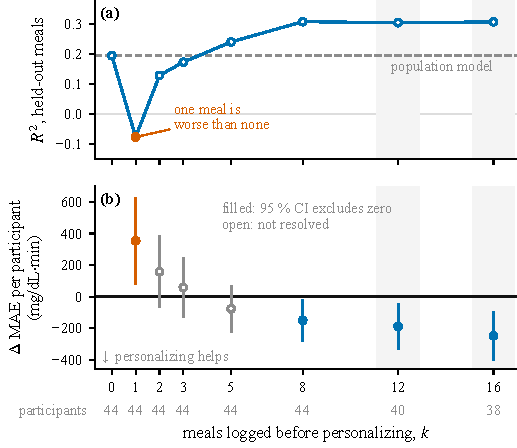
\includegraphics[width=\columnwidth]{fig1_personalisation.pdf}
\caption{Personalization from the first $k$ meals in time order, adapting the
output bias only, scored on each participant's remaining meals. (a)~Pooled
$R^2$; the dashed line is the unpersonalized population model. (b)~The same
result per participant, as a paired change in mean absolute error with a
95\,\% confidence interval. Filled markers exclude zero. One meal is
significantly worse than none, and eight are significantly better. A
participant needs $k+6$ meals to be scored, so the cohort shrinks at $k=12$ and
$16$ (shaded), and those points do not cover the same people as the rest.}
\label{fig:personalisation}
\end{figure}

\section{Device Architecture}

\subsection{Datapath and Weight Streaming}

Proof computes a two-layer quantized network,
\begin{align}
h &= \mathrm{ReLU}\!\left(\mathrm{clamp}_{0}^{127}\!\left((W_1 x + b_1) \gg s_1\right)\right), \nonumber \\
y &= (W_2 h + b_2) \gg s_2 ,
\end{align}
over INT8 weights and activations with power-of-two requantization, so that
rescaling is an arithmetic shift. Every neuron in both layers is the same
saturating dot product over a serial $8\times8$ multiplier and a 24-bit
accumulator. Only the source of the activations differs. In layer~1 the host
supplies them, re-streaming the input vector once per hidden neuron so that the
vector need not occupy 48 flip-flops. In layer~2 the chip supplies them from
the hidden-activation register.

\subsection{Monotonicity Argument and Interface Failure}

Write the pipeline for one output as a composition of the four stages above.
Each stage is monotone in its input: multiplication by a constant of fixed
sign, \emph{saturating} summation, arithmetic right shift, and clamping.
Composing them, $y$ is non-decreasing in the carbohydrate input $x_c$ provided
that every hidden unit $j$ satisfies
\begin{equation}
W_1[j][c] \cdot W_2[j] \;\geq\; 0 ,
\label{eq:sign}
\end{equation}
which we call the \emph{sign condition}. Each unit either helps carbohydrate
raise the response, or opposes it on both sides.

Two details of that argument are load-bearing. A saturating sum is monotone and
a wrapping sum is not, which makes saturation a safety requirement here and not
just a numerical nicety. Rounding mode, by contrast, is a red herring, since
every standard mode is monotone.

\begin{figure}[t]
\centering
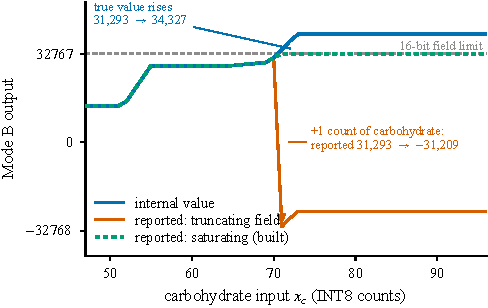
\includegraphics[width=\columnwidth]{fig2_r4_divergence.pdf}
\caption{The property held internally and broke at the pins. Carbohydrate is
swept for a weight set that \emph{satisfies} (\ref{eq:sign}). The internal
value never falls, but the truncating field wraps. Saturating the field
restores monotonicity end to end.}
\label{fig:r4}
\end{figure}

The argument covers the \emph{internal} value. The host never reads the
internal value. It reads a fixed-width field, and our output fields originally
truncated. Truncation wraps, and wrapping is emphatically not monotone. A
property-directed sweep found the reported response falling from 31{,}293 to
$-31{,}209$ for a one-count rise in carbohydrate while the true internal value
rose to 34{,}327. This happened in 55 of 400 randomized weight sets, all of
which satisfied (\ref{eq:sign}) (Fig.~\ref{fig:r4}). No stimulus-driven test
was going to surface it. Every result was bit-exact against the integer
reference model, because the reference truncated too; both were wrong in the
same way, so comparing them proved only that they agreed. Both fields now
saturate, which is monotone, and the same study reports 0 of 400.

\subsection{On-Chip Precondition Check}
\label{sec:guard}

\begin{figure*}[t]
\centering
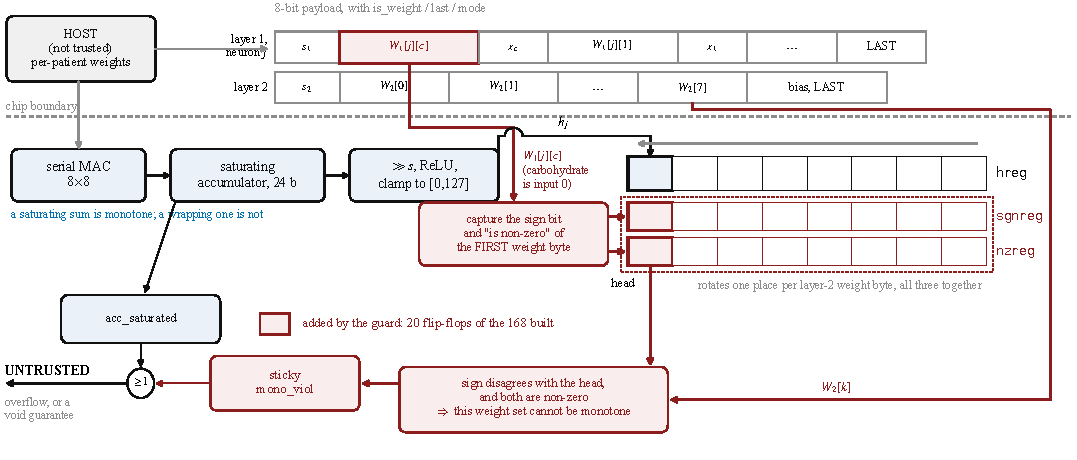
\includegraphics[width=\textwidth]{fig3_architecture.pdf}
\caption{Where the guard sits. Both operands of the sign condition
(\ref{eq:sign}) already cross the pins, but they cross at different times.
$W_1[j][c]$ is the first weight byte of hidden neuron $j$, while $W_2[j]$
arrives much later, in layer~2. Instead of storing a weight, the guard keeps
one sign bit (\texttt{sgnreg}) and one non-zero bit (\texttt{nzreg}) per hidden
unit in registers that rotate in lockstep with the hidden activations
(\texttt{hreg}). The bits for the unit being consumed therefore reach the head
exactly when that unit's layer-2 weight arrives. The hop marks wires crossing
without connecting.}
\label{fig:arch}
\end{figure*}

Condition (\ref{eq:sign}) is a property of the weights and not of the RTL, so a
device handed a fresh weight set for every patient cannot inherit an offline
certificate computed elsewhere. The chip therefore evaluates the condition
itself, in hardware, as the weights arrive.

The mechanism is cheap because both operands already cross the pins. The only
difficulty is that they arrive far apart in time. Carbohydrate is input~0 by
convention, so $W_1[j][c]$ is the \emph{first} weight byte of hidden neuron
$j$, while its partner $W_2[j]$ is the $j$-th weight byte of layer~2 and
arrives many bytes later. Storing the weights in order to compare them would
cost more than the datapath does. The guard instead stores one bit of each: the
sign of $W_1[j][c]$, and whether that weight is non-zero. These live in two
8-bit registers that rotate in \emph{lockstep} with the hidden-activation
register. Layer~2 consumes activations from the head of that register, so the
matching sign and non-zero bits reach the head of theirs at the same moment,
and the comparison reduces to an XOR, an eight-input OR reduction and three
ANDs (Fig.~\ref{fig:arch}).

Two subtleties are worth stating, since both are directly tested. A unit may
oppose carbohydrate on both sides, and two negative weights give a non-negative
product, so a naive ``all weights positive'' check would reject valid models. A
\emph{zero} carbohydrate weight can never violate the condition either, which
is why a non-zero bit is carried beside each sign.

The sticky flag is merged with the accumulator's saturation flag onto a single
output pin, since all eight pins were allocated already. \texttt{UNTRUSTED}
therefore means either numeric overflow \emph{or} a weight set that does not
admit the guarantee. To a caller the two mean the same thing, and the host
holds the weights, so it can always tell which.

The guard covers carbohydrate only. We built and measured a second guard for
the fiber direction and then declined it. It came to 187 flip-flops against
168, extrapolating to roughly 87\,\% utilization, which is too close to the
edge, and it buys the weaker of the two claims. The direction of the fiber
effect is domain knowledge that our data supports only marginally
($r=-0.051$). That guarantee still relies on the host using a constrained
objective.

\section{Dataset and Model Training}

We use CGMacros~\cite{cgmacros}, which covers 45 participants with concurrent
continuous glucose monitoring and photographed, macronutrient-labeled meals.
The dataset is public and de-identified, so this secondary analysis required no
new ethical approval. Our target is the two-hour incremental area under the
glucose curve. Splits are grouped by participant throughout, because a random
row split would place one person's meals on both sides and inflate every
number, since individual response varies most.

Two undocumented data-quality problems needed handling. \texttt{Meal Type}
carries ten label strings for four meal types, so filtering on
\texttt{== 'Breakfast'} silently discards 61\,\% of breakfasts. Separately, 52
records (3.0\,\%) exceed the dataset's own published maxima; a single fiber
entry of 2830~g against a documented maximum of 176 was enough on its own to
lift the training standard deviation for fiber to 32~g against a median of
3~g. Filtering against the published ranges improves out-of-fold $R^2$ from
$+0.215$ to $+0.225$.

One further property is documented in the dataset and not discovered here.
CGMacros breakfasts and lunches are standardized, and the 383 usable breakfasts
contain only 6 distinct macronutrient combinations. A breakfast-only analysis
would therefore be a \emph{personalization} study rather than a
meal-composition study, so we train across all meal types.

The model takes six meal features---carbohydrate, fiber, fat, protein, pre-meal
glucose and time of day---with eight hidden units. Participant-level biological
features are free in hardware, since the input count is not fixed in silicon,
but they do not earn their place. Adding A1c, BMI, age, fasting glucose and
insulin together collapses $R^2$ from $+0.225$ to $-0.014$, each of them being
fitted from 45 points. A1c alone raises population $R^2$ to $+0.256$ and barely
moves the median within-person correlation, but it \emph{reduces} the number of
participants ranked in the right direction from 41 to 37, and ranking is the
use case. No hidden width between 4 and 12 is distinguishable from 8 for the
constrained model that ships, so the model is data-limited rather than
capacity-limited. Quantization scales were selected by search over a held-out
fold, giving a mean float-to-INT8 error of 85 and a 95th percentile of 180
mg/dL$\cdot$min over 265 held-out meals, against a cohort mean response of
3150. The maximum error is 7305, on a single meal.

We train monotone models by reparameterization instead of by penalty, so the
constraint holds exactly at every step. For a constrained input $i$ with
required direction $s_i$ and a per-unit direction $d_j \in \{\pm 1\}$, we set
$W_1[j][i] = s_i d_j\,\mathrm{softplus}(A[j][i])$ and
$W_2[j] = d_j\,\mathrm{softplus}(c_j)$. Their product has sign exactly $s_i$
for every unit.

\section{Results}
\label{sec:results}

\subsection{Effect of Per-Patient Adaptation}

Fig.~\ref{fig:personalisation} sweeps the number of meals a person logs before
their model is adapted, refitting only the output bias. That is one parameter,
and one the chip already supports, since the host streams the bias as two
ordinary weight bytes. Meals are taken in time order, because sampling
someone's future to predict their past would inflate the result.

Personalization has a cost of entry. Calibrating on a single noisy meal moves
pooled $R^2$ from $+0.194$ to $-0.077$ and \emph{significantly harms}
per-participant error ($+354$ [$+77$, $+631$] mg/dL$\cdot$min). Break-even is
near five meals. At eight meals, roughly three days of logging, the paired
improvement is $-150$ [$-285$, $-16$] mg/dL$\cdot$min, 32 of 44 participants
improve, and pooled $R^2$ reaches $+0.307$.

One parameter is the right number. An affine calibration $y' = ay + b$ stays
closed-form and preserves monotonicity provided $a \geq 0$, yet at $k=2$ it
performs 1870 mg/dL$\cdot$min \emph{worse} than bias-only adaptation. It also
shows the constraint is not academic. At $k=2$ the fitted slope had to be
clamped at zero for 18 of 44 participants, so an unconstrained least-squares
calibration would have returned a negative slope and silently inverted the
model for 41\,\% of them.

\subsection{Precondition Satisfaction Under Per-Person Refitting}

Streaming weights per patient means a different weight set per patient, so the
question is whether a realistic per-person fit satisfies (\ref{eq:sign}). We
train a population model without constraints on the other participants,
warm-start from it, and continue training on one held-out participant's own
meals. This is the most ordinary thing a host would do, and it is deliberately
generous, because the refit sees all of that person's meals rather than the
eight that the curve above argues for.

In this cohort the refit never satisfies the condition. All 44 scored
participants yield a violating weight set, with a median of 3 offending hidden
units out of 8, and this is unchanged across fine-tuning budgets from 20 to 400
epochs. The population model already violates (\ref{eq:sign}) before any
personalization occurs. Personalization is not what breaks the condition; it is
what makes the condition undecidable offline, because the weight set the device
runs is not the one anyone certified.

The guard is therefore not redundant with our own training. Bias-only
adaptation cannot violate (\ref{eq:sign}), since it moves $b_2$ alone, whereas
full refitting can violate it and here always does. Nothing in the stream
distinguishes the two cases, which is why the check belongs at the interface.
\texttt{UNTRUSTED} marks a stream that has left the constrained path. It is not
a verdict on the patient.

\subsection{Accuracy Cost of the Monotonicity Constraint}

Under grouped 5-fold cross-validation, paired across folds, constraining
carbohydrate costs $-0.007$ $R^2$ with a 95\,\% confidence interval of
$[-0.033, +0.020]$. Adding the fiber direction costs $-0.025$
$[-0.062, +0.013]$. \textbf{No cost was detected, which is not the same as
free.} The interval admits a cost as large as $0.033$~$R^2$, so the honest
statement is that this study is underpowered to resolve a difference that
small.

For the same reason we do \emph{not} claim to beat the baseline. A depth-1
gradient-boosted baseline scores $0.059$~$R^2$ \emph{below} the unconstrained
network, at $[-0.118, -0.001]$. That interval barely excludes zero, and it does
not survive correction for the roughly ten comparisons made across this
project.

\subsection{Clinical Behavior}

Cross-fitting so that all 45 participants are held out exactly once (1308
meals), out-of-fold $R^2$ is $+0.225$. That figure is modest. Six meal
features, grouped splits, all meal types, no held-out cohort. The use case is
within-person ranking, where the median Spearman correlation is $+0.382$
(IQR $+0.215$ to $+0.495$), positive in 41 of the 44 participants with enough
meals to score. Broken out by glycemic status using ADA A1c thresholds, $R^2$
is $+0.074$ for 15 healthy, $+0.077$ for 16 pre-diabetic and $+0.142$ for 14
type~2 diabetic participants, while mean absolute error rises from 1557 to 2329
mg/dL$\cdot$min. Error grows with severity, but so does the response being
predicted.

\subsection{Implementation and Verification}

\begin{table}[t]
\caption{Implementation, IHP SG13G2, $1\times1$ Tiny Tapeout tile.
Latency 896 cycles $=$ 17.9\,\textmu s and 32.0\,nJ at 50\,MHz, so
35.1\,\textmu J for three meals a day for a year.}
\label{tab:silicon}
\centering
\footnotesize
\begin{tabular}{lrr}
\toprule
 & no guard & \textbf{as built} \\
\midrule
Flip-flops                 & 148       & \textbf{168} \\
Standard cells             & 1330      & \textbf{1443} \\
Utilization                & 76.35\,\% & \textbf{83.53\,\%} \\
DRC / LVS / antenna        & 0         & \textbf{0} \\
\bottomrule
\end{tabular}
\end{table}

Table~\ref{tab:silicon} gives the implementation result along with the guard's
marginal cost: 20 flip-flops and 113 standard cells, which takes utilization
from 76.35\,\% to 83.53\,\%. At that occupancy the tile is full, and that is
why the second guard was declined rather than built. The energy figure follows
from the place-and-route power estimate at the nominal corner together with the
measured cycle count, so it inherits the tool's switching-activity assumptions.

Verification is 43 top-level tests, all bit-exact against an integer reference
model, of which 6 are \emph{exhaustive} over all 65{,}536 signed $8\times8$
multiplier inputs. All 54 named coverage bins are hit, and each is asserted
rather than printed. Of 29 mutants none escape: 28 are caught and 1 is proven
equivalent by the exhaustive test. Gate-level simulation also runs with the
post-route SDF back-annotated at all three corners, where the same 43 tests
pass against real cell and interconnect delays. Our simulator implements no
timing checks, so setup and hold still rest on static analysis alone.

\section{Limitations}

\textit{Selection bias is the dominant limitation.} Quantization scales, hidden
width, adaptation method and constraint set were all chosen while looking at
the same cross-validation folds that the results are reported on. Forty-five
participants was not enough to hold a clean cohort back. Every absolute figure
here is therefore optimistically biased and should be read as an upper bound.
The paired comparisons, which share folds and models, are the more trustworthy
quantities.

\textit{The study is underpowered} for the effects it measures. Nothing
reported here survives correction for the number of comparisons made across the
project. That is why we claim no cost \emph{detected} instead of no cost, and
why we claim no advantage over the baseline at all.

\textit{The truncation defect is not reachable on our data.} With real trained
weights, zero of 265 held-out meals overflow the 16-bit field at any
requantization shift from 0 to 6. The defect is real and appears in 55 of 400
synthetic weight sets, but we make no claim of patient harm on real data.

\textit{The guard covers one of the two claimed directions,} as discussed in
Section~\ref{sec:guard}. The chip is a $1\times1$ tile on a shared
multi-project wafer, and what we report is pre-silicon signoff, not measurement
from returned parts.

\textit{Novelty is asserted} on the basis of six literature searches, which is
weak evidence.

\textit{This is not a medical device.} Every output is an estimate.

\section{Conclusion}

A monotonicity guarantee is a property of a weight set, and a device handed a
new weight set for every patient cannot inherit a certificate computed for
someone else's. The failure is not hypothetical: an unconstrained per-person
refit violates the sign condition in 44 of 44 cases in this cohort. The
precondition is nonetheless checkable at the interface for 20 flip-flops,
because both operands already cross the pins. A guarantee of this kind can also
hold throughout a datapath and still be destroyed by the fixed-width field that
reports it.

RTL, testbenches, reference models and the scripts that regenerate every figure
here are at \url{https://github.com/kush1434/proof}. Trained weights are
excluded, because CGMacros is CC~BY-NC-SA and the repository is Apache-2.0.

\begin{thebibliography}{15}

\bibitem{liu2020}
X. Liu, X. Han, N. Zhang, and Q. Liu, ``Certified monotonic neural networks,''
in \emph{Advances in Neural Information Processing Systems (NeurIPS)}, vol.~33,
2020.

\bibitem{runje2023}
D. Runje and S.~M. Shankaranarayana, ``Constrained monotonic neural networks,''
in \emph{Proc. 40th Int. Conf. Machine Learning (ICML)}, PMLR vol.~202, 2023.

\bibitem{scalable2024}
H. Kim and J.-S. Lee, ``Scalable monotonic neural networks,'' in \emph{Proc.
Int. Conf. Learning Representations (ICLR)}, 2024.

\bibitem{quantmon2026}
J. Li, P.~H.~W. Leong, and T. Chaffey, ``Quantization robustness of monotone
operator equilibrium networks,'' \emph{arXiv:2603.10562}, 2026.

\bibitem{qvip2022}
Y. Zhang, Z. Zhao, G. Chen, F. Song, M. Zhang, T. Chen, and J. Sun, ``QVIP: An
ILP-based formal verification approach for quantized neural networks,'' in
\emph{Proc. 37th IEEE/ACM Int. Conf. Automated Software Engineering (ASE)},
2022.

\bibitem{huang1984}
K.-H. Huang and J.~A. Abraham, ``Algorithm-based fault tolerance for matrix
operations,'' \emph{IEEE Trans. Computers}, vol.~C-33, no.~6, pp.~518--528,
1984.

\bibitem{ozen2020}
E. Ozen and A. Orailoglu, ``Low-cost error detection in deep neural network
accelerators with linear algorithmic checksums,'' \emph{J. Electronic Testing:
Theory and Applications}, vol.~36, pp.~703--718, 2020.

\bibitem{zhang2018}
J.~J. Zhang, T. Gu, K. Basu, and S. Garg, ``Analyzing and mitigating the impact
of permanent faults on a systolic array based neural network accelerator,'' in
\emph{Proc. IEEE 36th VLSI Test Symposium (VTS)}, 2018.

\bibitem{putra2022}
R.~V.~W. Putra, M.~A. Hanif, and M. Shafique, ``SoftSNN: Low-cost fault
tolerance for spiking neural network accelerators under soft errors,'' in
\emph{Proc. 59th ACM/IEEE Design Automation Conference (DAC)}, 2022.

\bibitem{xiang2022}
W. Xiang, ``Runtime safety monitoring of neural-network-enabled dynamical
systems,'' \emph{IEEE Trans. Cybernetics}, vol.~52, no.~9, pp.~9587--9596,
2022.

\bibitem{zeevi2015}
D. Zeevi, T. Korem, N. Zmora, et al., ``Personalized nutrition by prediction of
glycemic responses,'' \emph{Cell}, vol.~163, no.~5, pp.~1079--1094, 2015.

\bibitem{berry2020}
S.~E. Berry, A.~M. Valdes, D.~A. Drew, et al., ``Human postprandial responses
to food and potential for precision nutrition,'' \emph{Nature Medicine},
vol.~26, no.~6, pp.~964--973, 2020.

\bibitem{cgmacros}
A. Das, D. Kerr, N. Glantz, W. Bevier, R. Santiago, R. Gutierrez-Osuna, and
B.~J. Mortazavi, ``CGMacros: A pilot scientific dataset for personalized
nutrition and diet monitoring,'' \emph{Scientific Data}, vol.~12, art.~1557,
2025.

\bibitem{tinytapeout}
M. Venn, ``Tiny Tapeout: A shared silicon tape out platform accessible to
everyone,'' \emph{IEEE Solid-State Circuits Magazine}, vol.~16, no.~2,
pp.~20--29, 2024.

\bibitem{ihp}
IHP, ``SG13G2 open source PDK,''
\url{https://github.com/IHP-GmbH/IHP-Open-PDK}.

\end{thebibliography}

\end{document}
